\documentclass[sigconf,screen,nonacm]{acmart}
\settopmatter{printacmref=false, printccs=false, printfolios=true}
\setcopyright{none}
\renewcommand\footnotetextcopyrightpermission[1]{}
\renewcommand{\shortauthors}{}
\providecommand\acmBooktitle{}
\renewcommand\acmBooktitle{}
\pagestyle{plain}
\raggedbottom

\usepackage{listings}
\usepackage{xcolor}
\usepackage{tcolorbox}
\usepackage{graphicx}
\graphicspath{{./}{../reports/}}

\makeatletter
\def\@typeset@author@bx{\bgroup\hsize=\author@bx@wd
  \def\and{\par}\normalbaselines
  \global\setbox\author@bx=\vtop{\centering
    \@authorfont\@currentauthors}\egroup
  \box\author@bx\hspace{\author@bx@sep}%
  \gdef\@currentauthors{}%
  \gdef\@currentaffiliation{}}
\makeatother

\AtBeginDocument{%
  \providecommand\BibTeX{{%
    Bib\TeX}}}

\begin{document}

\title{Scheduling and Execution Granularity for GPU Logic Simulation}

\author{Jianing Ou, Xuechun Jin, Yayen Lin, and Matthew Kearney}
\affiliation{%
  \institution{University of Wisconsin-Madison}
  \city{Madison}
  \state{WI}
  \country{USA}}
\renewcommand{\authorsaddresses}{}


\begin{abstract}
GPU logic simulation contains many fine-grained gate-level operations with strict data dependencies. Although gates on the same dependency frontier can execute in parallel, each individual gate has very little computation, so CUDA kernel launch overhead, host-side scheduling overhead, and dependency update overhead can easily exceed the actual computation cost. This paper studies the tradeoff between scheduling policy and execution granularity for circuit task graph execution on GPUs. We construct DAGs from ISCAS-style benchmark circuits, compare four gate-level scheduling policies, and evaluate both batch blocking and batch non-blocking execution modes. We also implement levelization and fused levelization, which raise the execution unit from a gate batch to a topological level or fused levels in order to reduce the overhead caused by overly fine-grained scheduling. The experimental results show that gate-level scheduling is not suitable for executing circuit graphs because of large host-side bookkeeping and kernel launch overhead. In contrast, levelization significantly reduces the number of scheduling units and the cost of dependency updates, leading to clear performance improvements across small, medium, and large circuits. Fused levelization further mitigates repeated kernel launches caused by narrow tail levels. Overall, for fine-grained and dependency-heavy GPU logic simulation workloads, choosing an appropriate execution granularity is more important than designing a more complex gate-level scheduler.
\end{abstract}
\maketitle

\section{Introduction}
Logic simulation is a central step in digital circuit verification. A circuit can naturally be represented as a directed acyclic graph (DAG), where each node is a logic gate and each edge represents a signal dependency. A gate can only execute after all of its predecessor gates have completed. GPUs provide massive parallelism, and gates at the same dependency level can potentially be evaluated in parallel. However, the computation performed by a single gate is very small. Basic logic operations such as AND, OR, XOR, and inversion require only a few instructions. As a result, launching too many small GPU kernels can make kernel launch overhead and synchronization overhead larger than the actual computation.

This project studies how scheduling policy and execution granularity affect GPU logic simulation. GPU scheduling is a long-standing problem in shared and real-time GPU systems, where non-preemptive execution can strongly affect latency and fairness \cite{kato2011timegraph}. We compare two major directions, shown in \autoref{fig:pipeline}. The first direction is gate-level scheduling, where each gate is a schedulable task and a scheduler selects ready gates from a ready queue. The second direction is levelized execution, where the circuit is first organized by topological levels and all gates in one level are executed as a coarser task. However, many circuits contain a long narrow tail: later levels may contain only a few gates. If one GPU kernel is launched for every narrow level, launch overhead can still dominate runtime. Therefore, we further implement fused levelization, which merges consecutive small levels into a single GPU kernel to reduce repeated launch overhead in narrow tail levels.

The main contributions are as follows. First, we implement and compare several gate-level scheduling policies, including FIFO, fanin priority, SJF, and dependency-aware scheduling, and evaluate different execution modes, including batch blocking and batch non-blocking. Second, we implement levelization and fused levelization with three fusion thresholds, and analyze performance across multiple benchmark circuits.

\begin{figure*}[t]
  \centering
  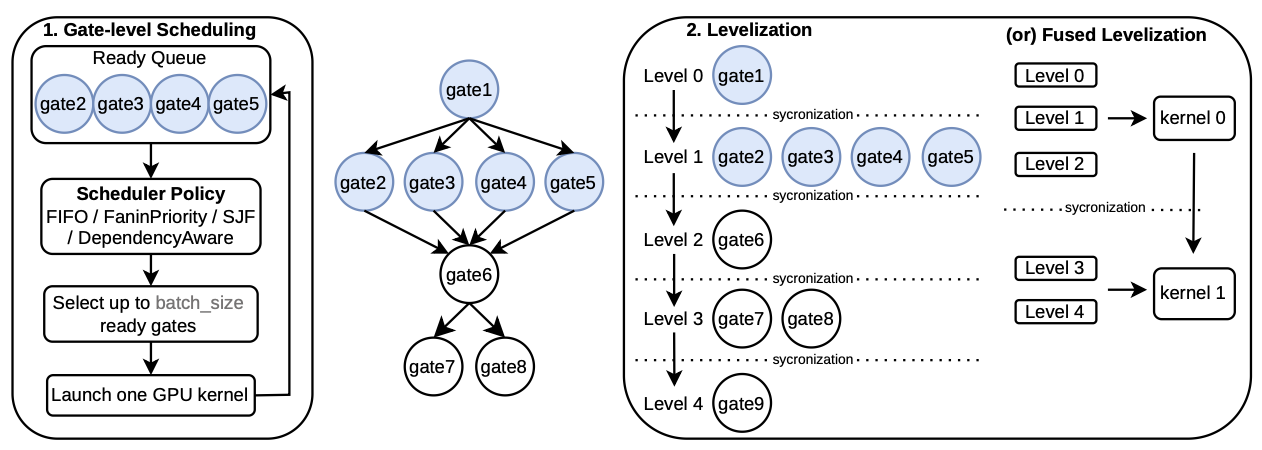
\includegraphics[width=0.8\textwidth]{Figure1.png}
  \caption{System Overview. Suppose the gate1 here in the circuit has been executed, and gate2/gate3/gate4/gate5 is ready to execute.}
  \label{fig:pipeline}
\end{figure*}

\section{Methodology}
\subsection{Circuit Parsing and Task Graphs}
We parse benchmark \texttt{.ckt} files to obtain gate counts, wire connections, gate types, and fan-in information. The circuit is stored as adjacency and inverse-adjacency lists. For gate-level scheduling, each gate is converted into a \texttt{Task} object storing its gate id, priority, dependency list, remaining dependency count, and timing fields. A task becomes ready when its remaining dependency count reaches zero.

For levelization, the same circuit DAG is transformed into a level-task graph. Source gates are placed at level 0, and every other gate is assigned to one plus the maximum level among its predecessors. All gates with the same level are packed into one level task. This representation changes the scheduling unit from an individual gate to an entire topological level.

\subsection{GPU Execution Backend}
The GPU executor uses a unified gate-batch kernel. After a scheduler selects a batch of gates, the host copies their gate ids to the GPU and launches one CUDA kernel. Inside the kernel, each CUDA thread maps to one gate id, reads gate type and fan-in metadata, gathers predecessor outputs, and computes the gate output. To make gate cost observable, we assign synthetic work units proportional to fan-in and repeat the gate computation accordingly.

Before each scheduler run, the executor resets gate outputs. Around each kernel launch, the host records launch and completion timestamps. These timestamps are used to compute host-side makespan and GPU busy intervals. GPU utilization is defined as the union of host-side active kernel intervals divided by makespan. This is a runtime-level utilization metric, not a profiler-level SM occupancy measurement.

\subsection{Scheduling Policies and Execution Modes}
We compare four gate-level scheduling policies. FIFO executes ready gates in submission order and serves as the simplest baseline. Fanin priority favors gates with larger fan-in. Shortest-Job-First (SJF) favors gates with smaller estimated work and is intended to reduce average waiting time. In our implementation, the estimated work is proportional to fan-in, so SJF effectively selects the ready gate with the smallest fan-in first. Dependency-aware scheduling precomputes the number of immediate downstream dependents for each gate and prioritizes gates that can potentially unlock more future work, i.e., gates with larger fan-out.

These policies are evaluated under two main gate-level execution modes. Batch blocking selects up to \texttt{batch\_size} ready gates, launches one gate-batch kernel, waits for the batch to finish, and then updates the dependencies of all completed gates in that batch. Successor gates are inserted into the ready queue as soon as they become ready.

This creates a clear batch-level barrier: no successor gate is submitted until the whole launched batch completes. Batch non-blocking keeps several batches in flight across CUDA streams. As long as a stream is free, the scheduler can launch another ready batch. When any in-flight batch finishes, the host updates the dependencies of gates in that batch and immediately submits newly ready gates back to the scheduler. This mode reduces idle gaps and improves dependency responsiveness, while still using batch kernels instead of launching every gate individually.

\subsection{Levelization and Fused Levelization}
Levelization converts the gate-level DAG into a level-task graph (Figure 1(c)). Each level task contains all gates in one topological level. The baseline levelization method launches one gate-batch kernel per level task and waits at level-wave barriers before unlocking later levels. Since gates in the same level are independent, this execution mode naturally exposes parallelism and reduces the number of scheduling units.

Fused levelization further merges consecutive small levels. Given a threshold \texttt{T}, if a ready level has no more than \texttt{T} gates, the scheduler continues checking the following levels from the same circuit. As long as each level is also under the threshold, the levels are placed into the same fused segment. The fused segment is processed by one CUDA kernel. The kernel iterates through levels in order, uses one thread block to process gates within each level, and uses \texttt{\_\_syncthreads()} between levels for lightweight intra-kernel synchronization. We evaluate \texttt{T = 256}, \texttt{T = 1024}, and \texttt{T = 2048}.

\section{Experimental Setup}
\subsection{Benchmarks}
The evaluation uses ISCAS-style benchmark circuits from the course-provided LSIM framework \cite{lsim}. The small circuits include \texttt{c17}, \texttt{c432}, \texttt{c499}, and \texttt{c880}. The medium circuits include \texttt{c1355}, \texttt{c1908}, \texttt{c2670}, and \texttt{c3540}. The large circuits include \texttt{c5315}, \texttt{c6288}, and \texttt{c7552}. Each circuit is evaluated independently, so the reported results focus on single-circuit execution behavior.

Gate-level experiments use batch sizes of 32, 128, and 512. Fused levelized experiments use \texttt{fused\_level(256)}, \texttt{fused\_level(1024)}, and \texttt{fused\_level(2048)}. Each configuration is repeated multiple times on a T4 GPU, and the final reported value is the average over runs.

\subsection{Metrics}
In our experiment, all the following indicators were measured. The main trends of the first three indicators and the changes in makespan in the analysis were roughly consistent. Therefore, in the analysis, we mainly focused on makespan, GPU utilization and throughput.

Average wait time measures how long a gate waits after becoming ready and before being launched. Maximum wait time is used as a starvation indicator.

Average execution time is the host-side service interval attributed to each gate. In batch execution, all gates in a batch share the batch service time. In levelization, all gates in a level share the level service time. In fused levelization, the fused segment service time is divided across levels in proportion to each level's gate count, preventing the entire fused segment time from being assigned repeatedly to every level.

Average turnaround time is wait time plus execution time.

Makespan is the total host-side runtime from the beginning of a scheduler run to the completion of the final GPU task.

Throughput is the number of completed gates divided by makespan.

GPU utilization is the union of host-side active GPU intervals divided by makespan.

\section{Results and Analysis}
\subsection{Gate-Level Batch Scheduling}
\begin{figure*}[t]
  \centering
  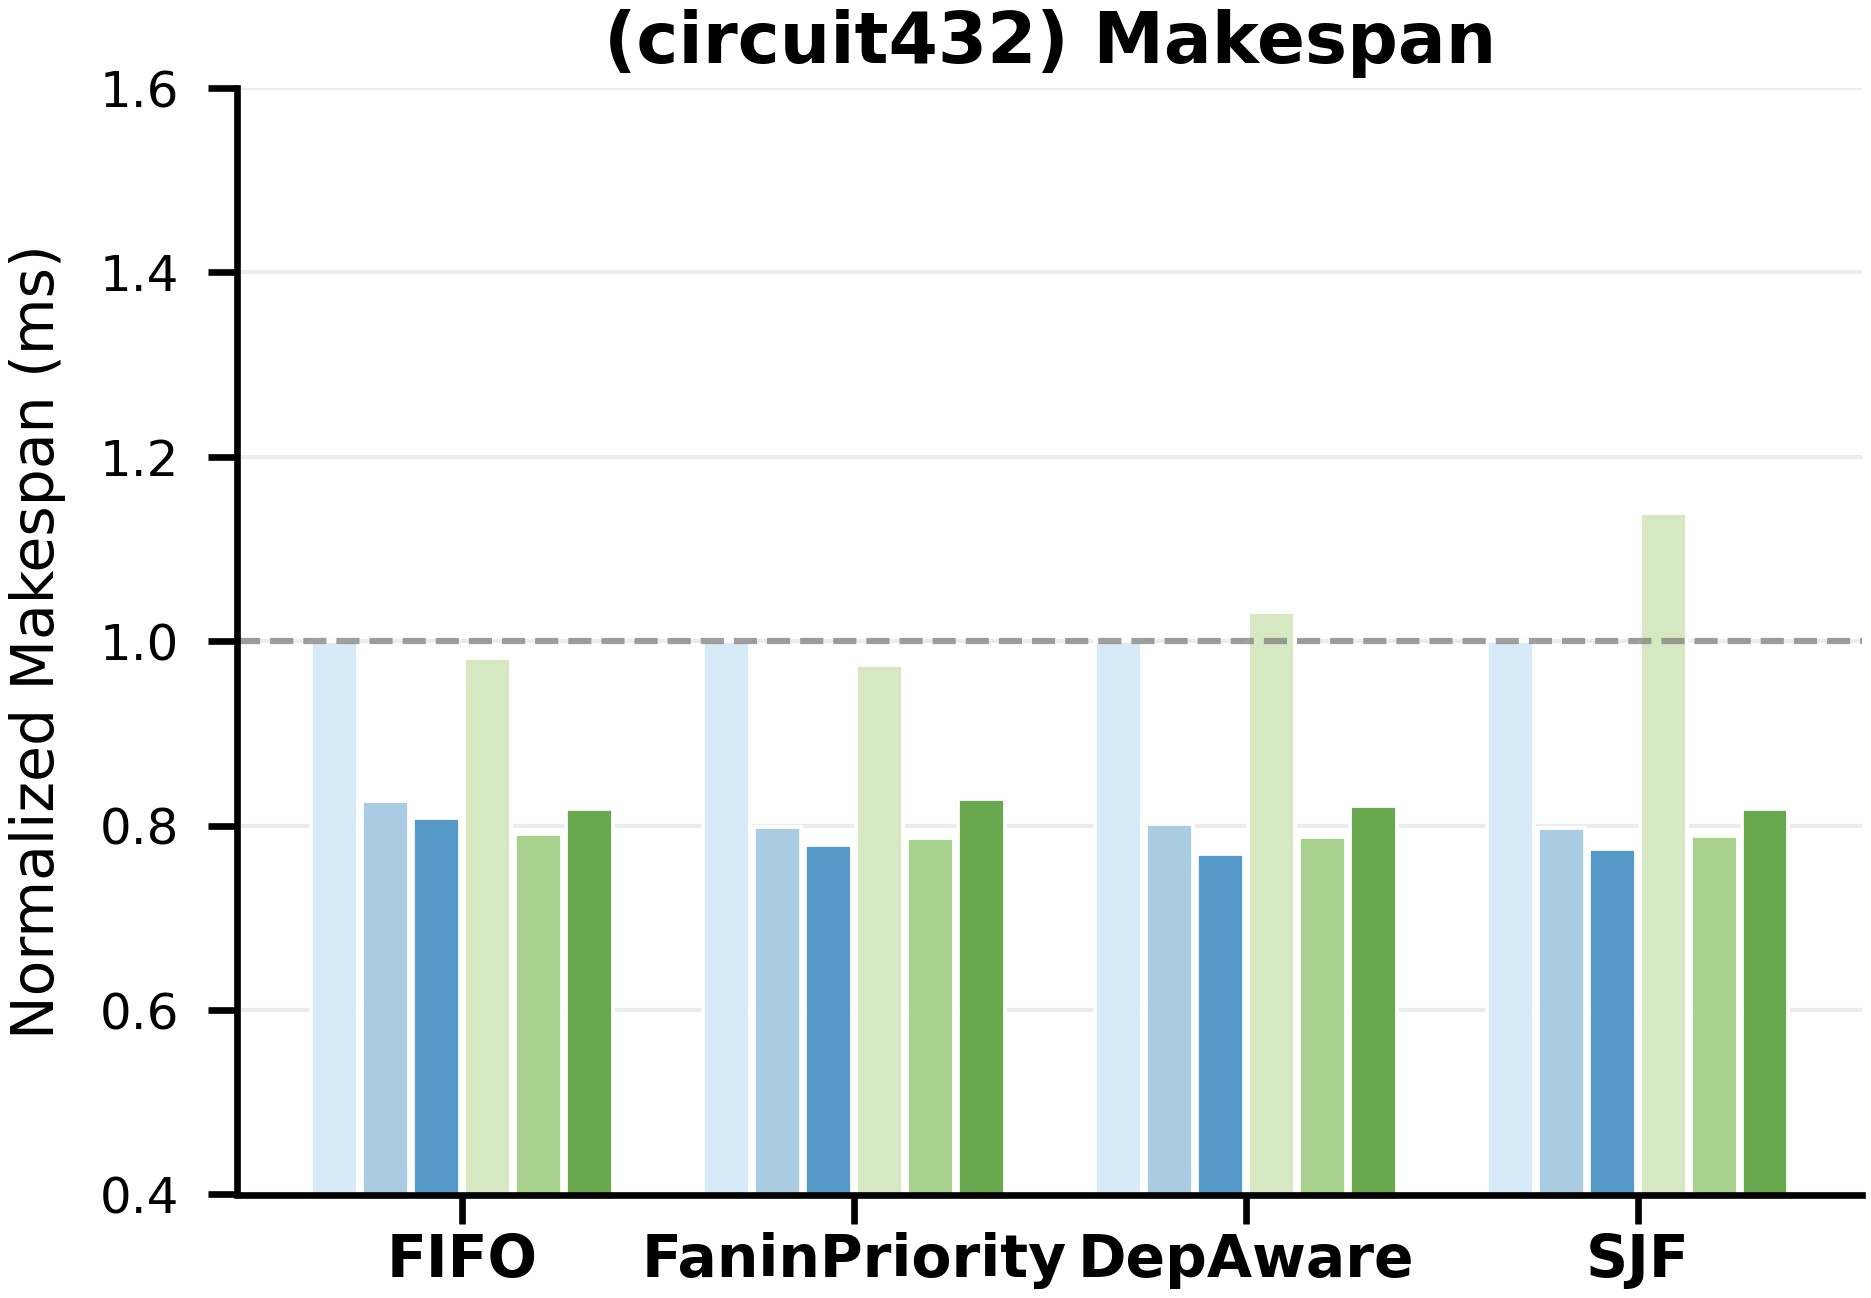
\includegraphics[width=0.31\textwidth]{report_c432_scheduling_makespan.png}
  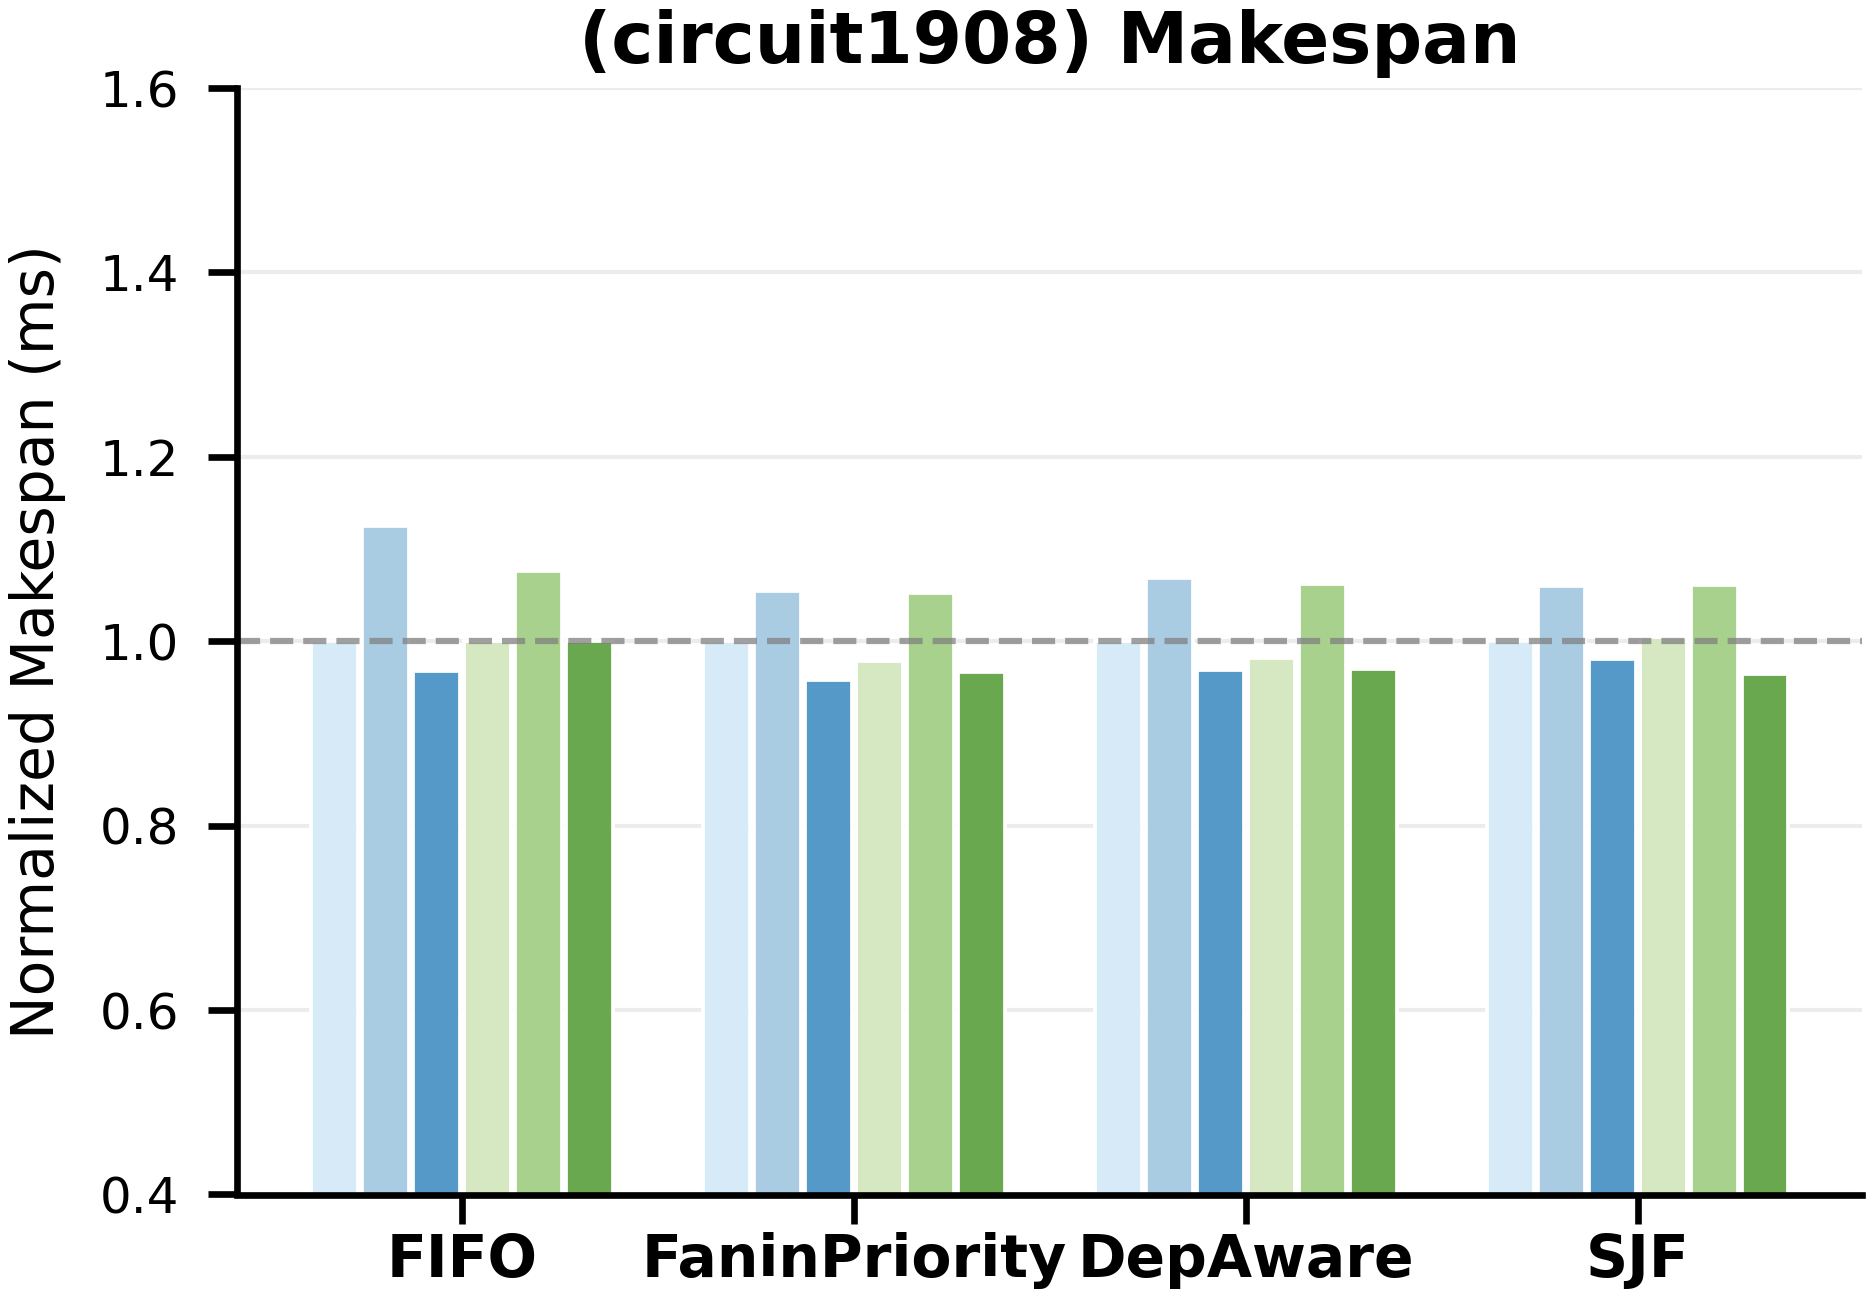
\includegraphics[width=0.31\textwidth]{report_c1908_scheduling_makespan.png}
  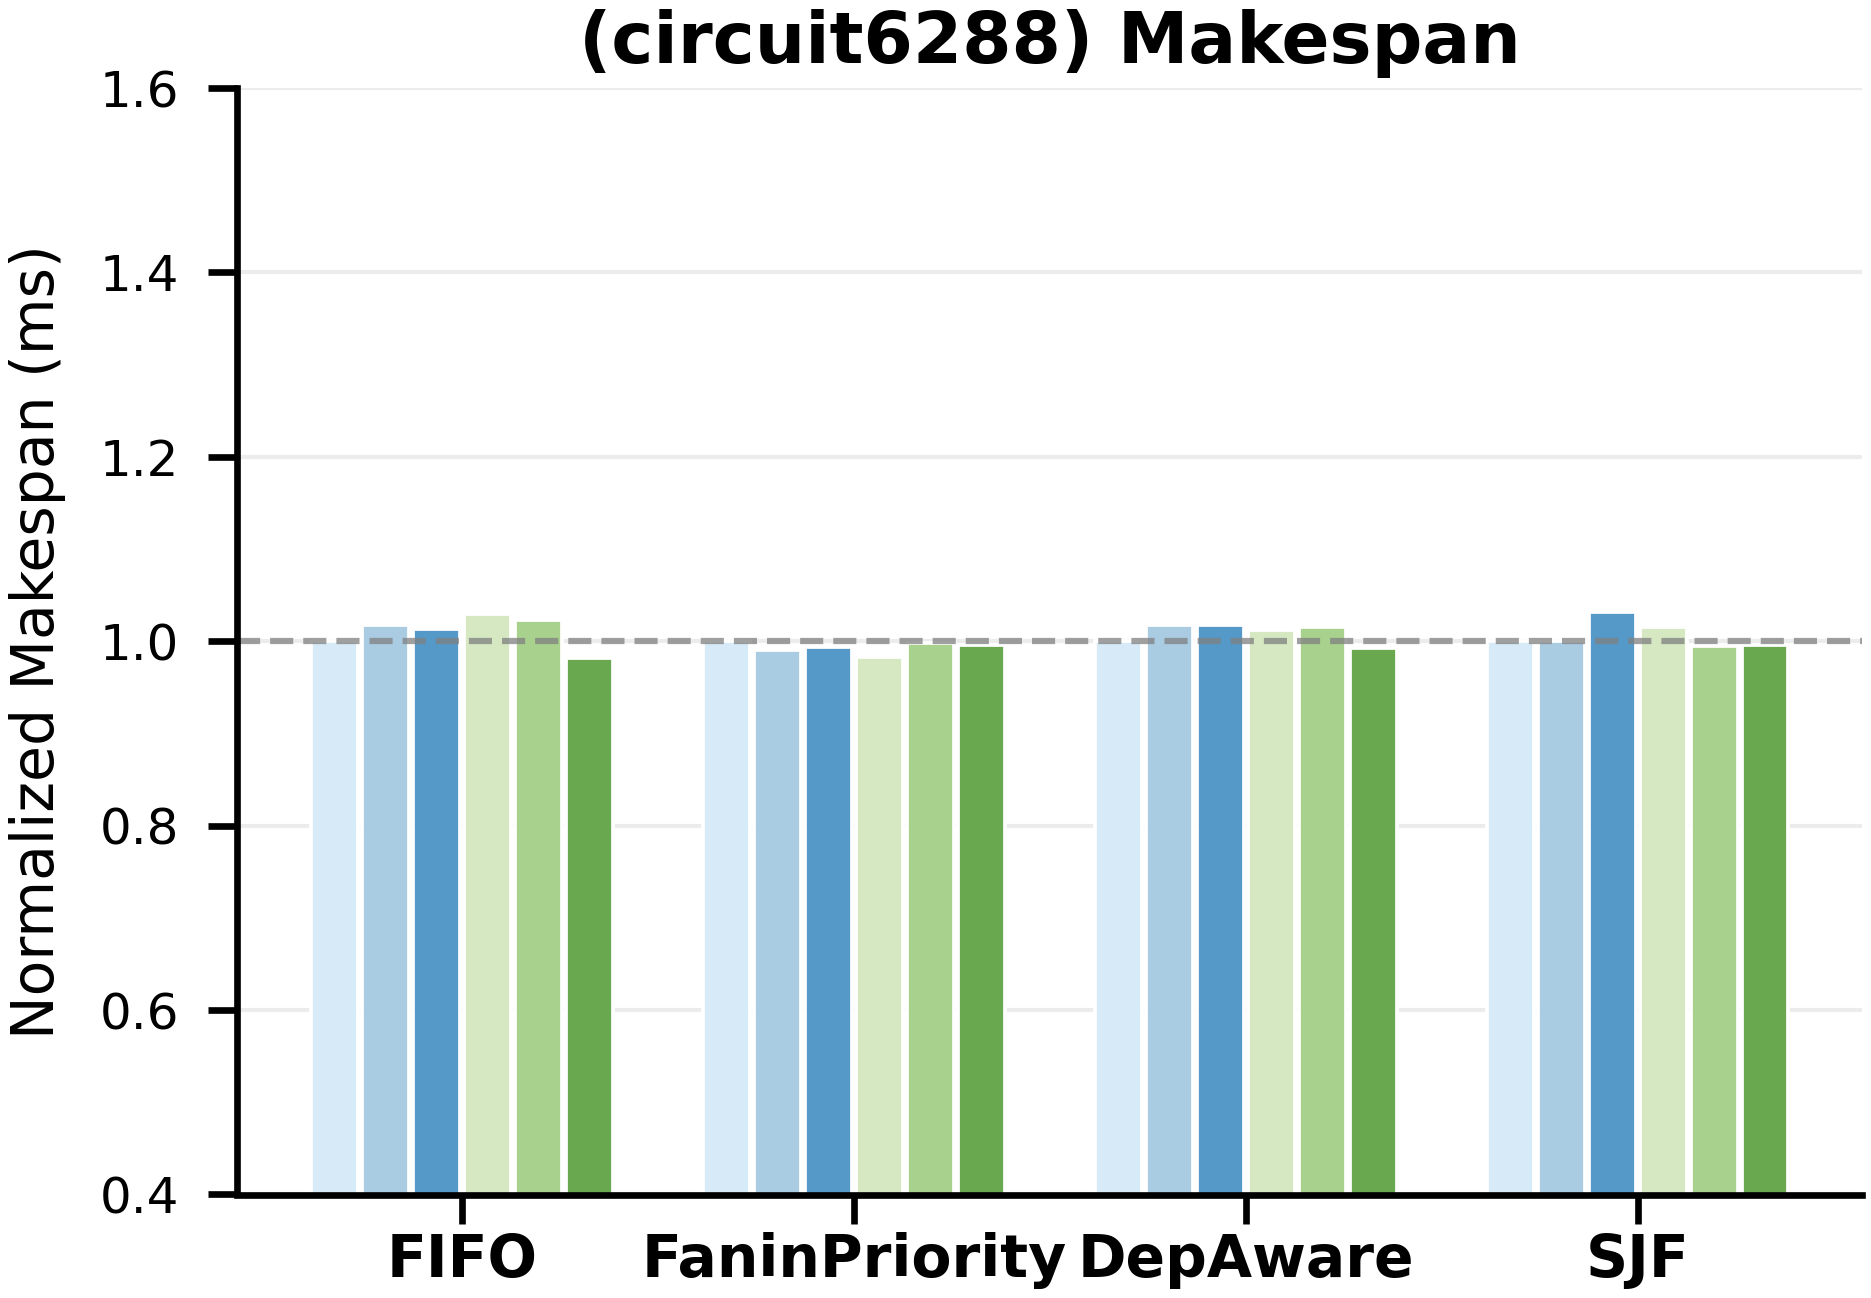
\includegraphics[width=0.31\textwidth]{report_c6288_scheduling_makespan.png}
  \par\vspace{3pt}
  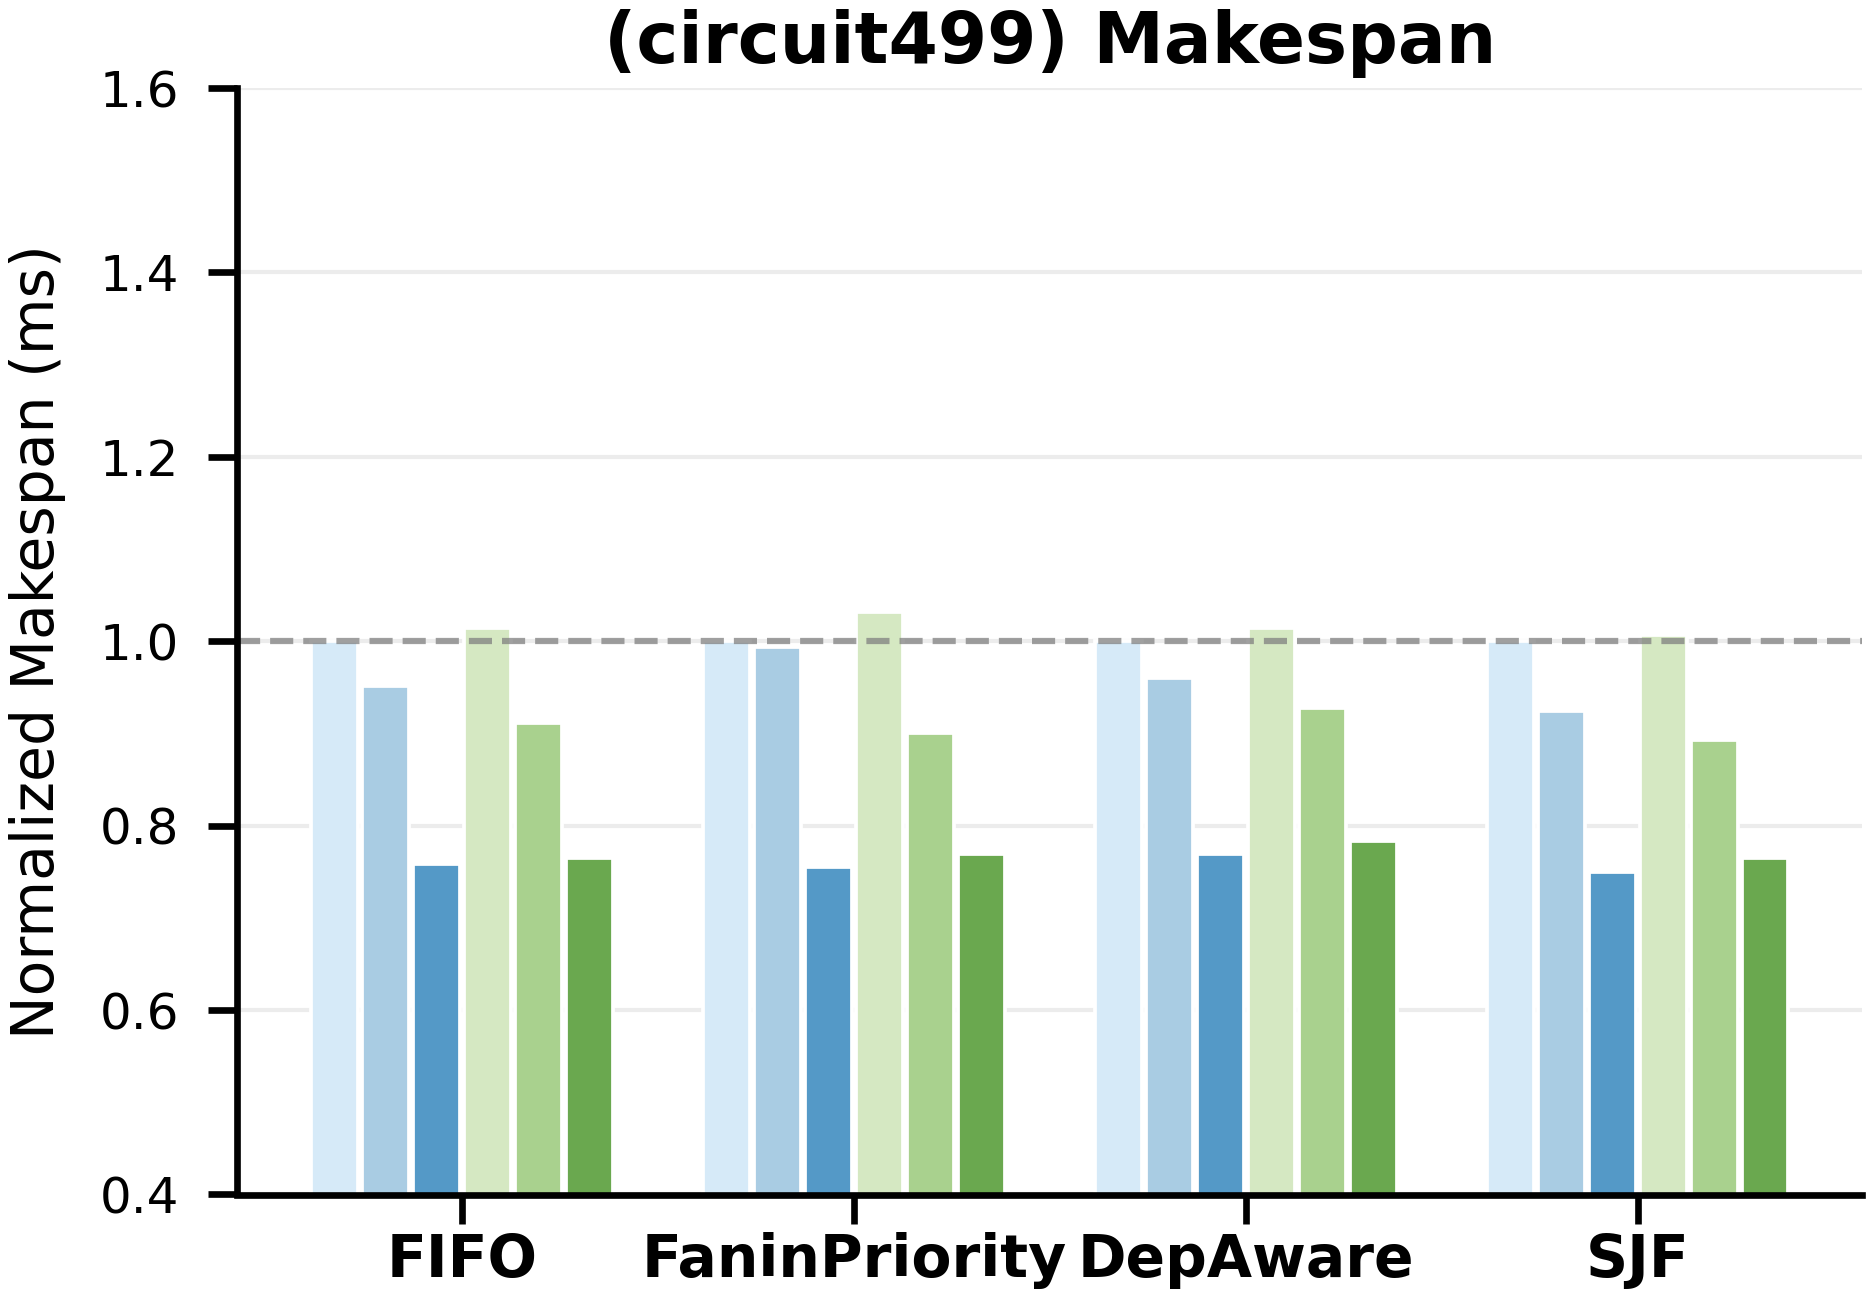
\includegraphics[width=0.31\textwidth]{report_c499_scheduling_makespan.png}
  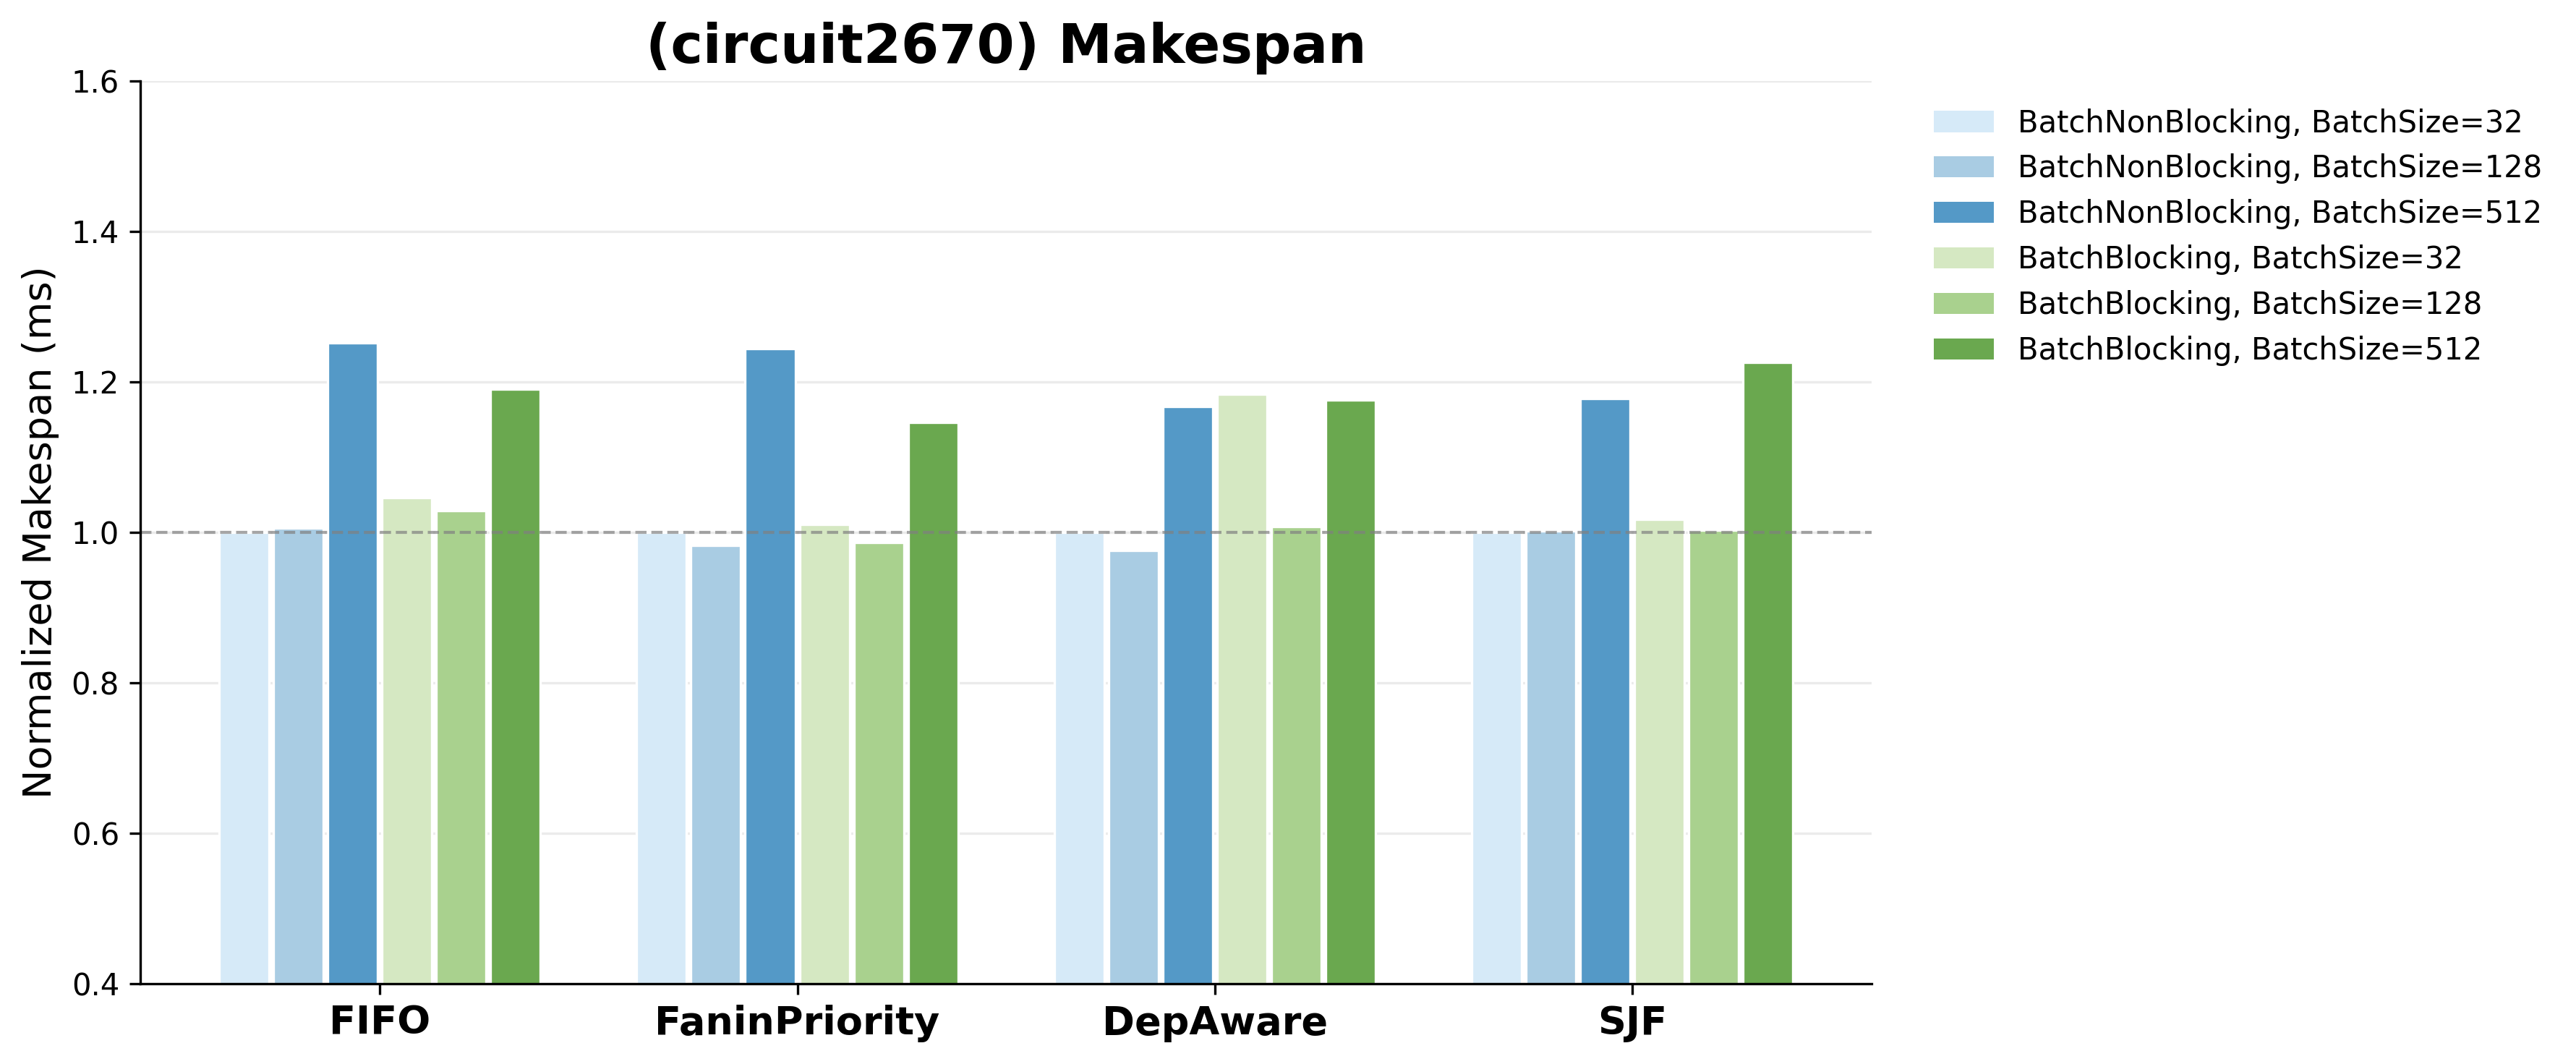
\includegraphics[width=0.31\textwidth]{report_c2670_scheduling_makespan.png}
  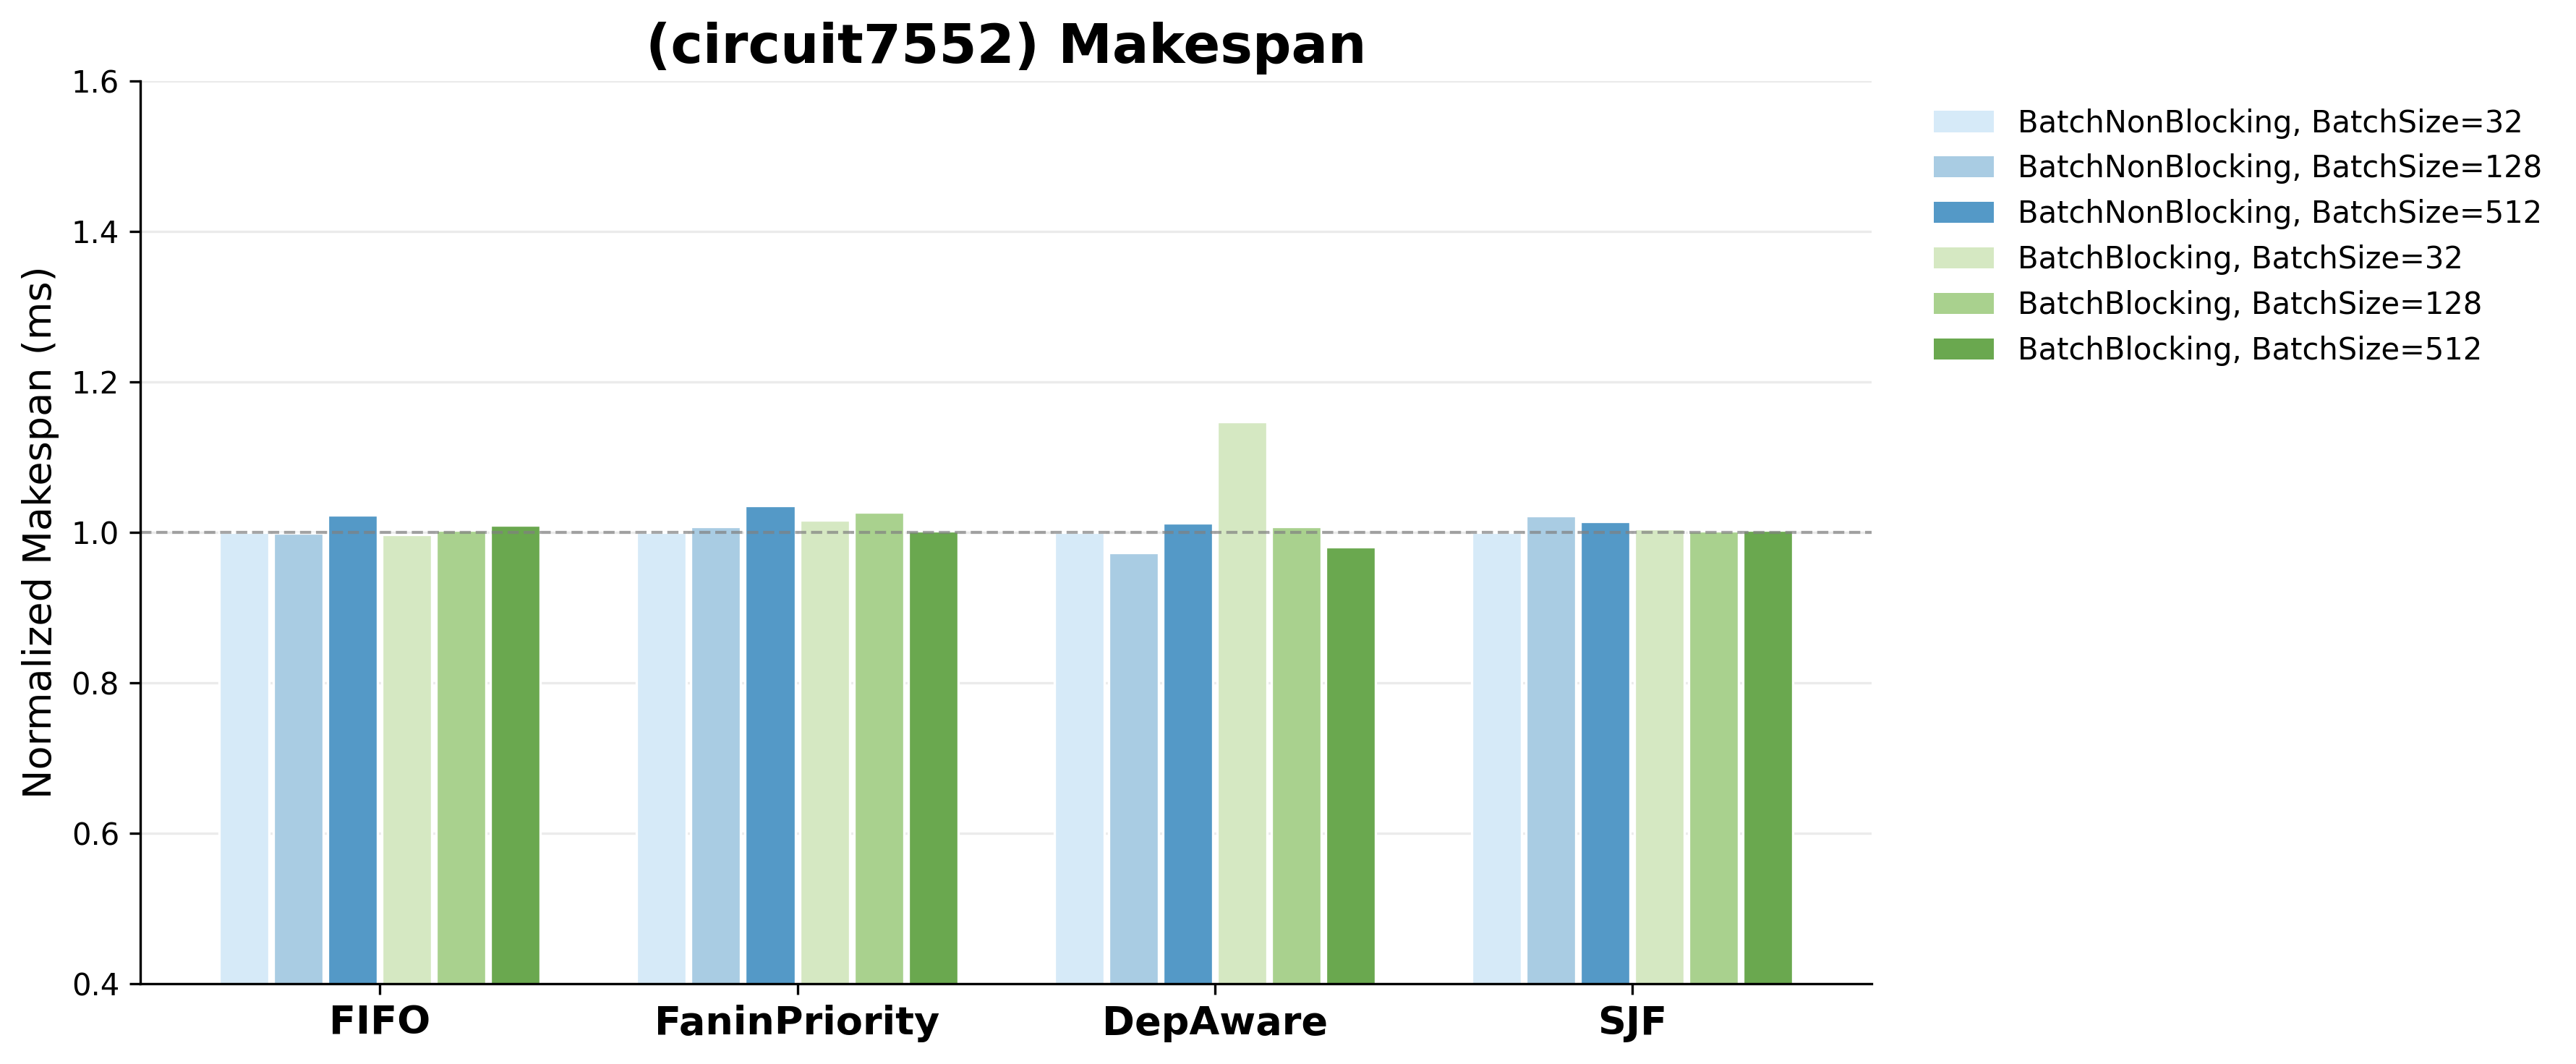
\includegraphics[width=0.31\textwidth]{report_c7552_scheduling_makespan.png}
  \par\vspace{1pt}
  \makebox[0.31\textwidth]{\small (a) small circuits}
  \makebox[0.31\textwidth]{\small (b) medium circuits}
  \makebox[0.31\textwidth]{\small (c) large circuits}
  \par\vspace{2pt}
  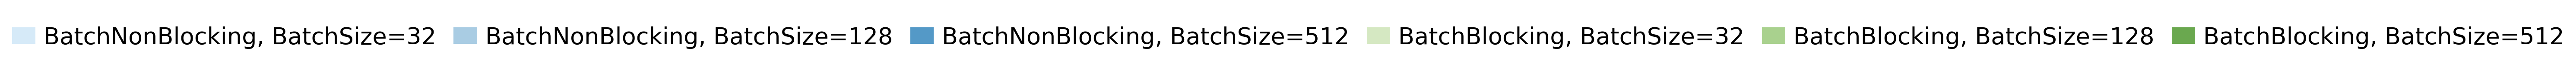
\includegraphics[width=1\textwidth]{legend.png}
  \caption{Gate-level scheduling across representative small, medium, and large circuits. Each bar is normalized to the FIFO batch blocking baseline with batch size 32.}
  \label{fig:scheduling}
\end{figure*}

We first compare different scheduling policies under batch blocking. The differences among policies are usually small for the same batch size. This is because each gate operation is extremely lightweight, so changing ready-queue ordering alone cannot compensate for launch overhead and dependency-update overhead, as explained further in \autoref{sec:fused-levelization}. Dependency-aware scheduling can help in some circuits by unlocking downstream gates earlier, but its benefit is limited when the ready set is already large or when launch overhead dominates.

Larger \texttt{batch\_size} does not always improve performance. For small circuits, increasing batch size can reduce the number of kernel launches and sometimes lower makespan. For example, in \texttt{c499} (\autoref{fig:scheduling}), FIFO non-blocking reduces makespan by about 25\% when \texttt{batch\_size} increases from 32 to 512. This suggests that, when the circuit is small and each gate has very low computation cost, launch overhead is a major bottleneck and larger batches can amortize that overhead. However, this trend is not stable for larger circuits. For example, in \texttt{c2670} (\autoref{fig:scheduling}), makespan increases for different scheduling policies when \texttt{batch\_size} increases from 128 to 512. We attribute this to two factors. First, under blocking execution, the host must wait until each batch completes before updating the dependent counts of completed gates and checking which successor gates become ready. In larger circuits, dependency updates and ready-queue maintenance are much larger in scale, so the coarse-grained progress and bursty updates caused by a large batch can offset or even exceed the reduction in launch overhead. Second, the ready frontier of a circuit is limited by the DAG topology, so there are not always enough ready gates to fill a large batch.

Batch non-blocking is designed to address a limitation of batch blocking: blocking execution must wait for the current batch to finish before dependency progress can continue. Non-blocking execution allows multiple batches to run concurrently on different CUDA streams and updates successors as soon as a batch completes. In theory, this should reduce GPU idle time and submit ready work earlier. However, in our experiments, the difference between non-blocking and blocking is still small. We attribute this to two reasons. First, although non-blocking can increase stream-level overlap, each gate computation is very lightweight, so the kernel execution time is short and the amount of GPU work that can be overlapped is limited. Second, the host still needs to frequently poll batch completion, update dependencies, maintain the ready queue, and submit new batches. If these CPU-side overheads and DAG bookkeeping costs dominate, adding multiple streams cannot significantly reduce makespan and may even introduce extra management overhead.

Therefore, the limited improvement from blocking to non-blocking suggests that optimizing only the batch dispatch mode is not enough. The more fundamental bottleneck is likely execution granularity: gate-level scheduling treats every gate as an individual task, which creates substantial scheduling overhead and host-side dependency maintenance.

\subsection{Levelization}
\begin{figure*}[t]
  \centering
  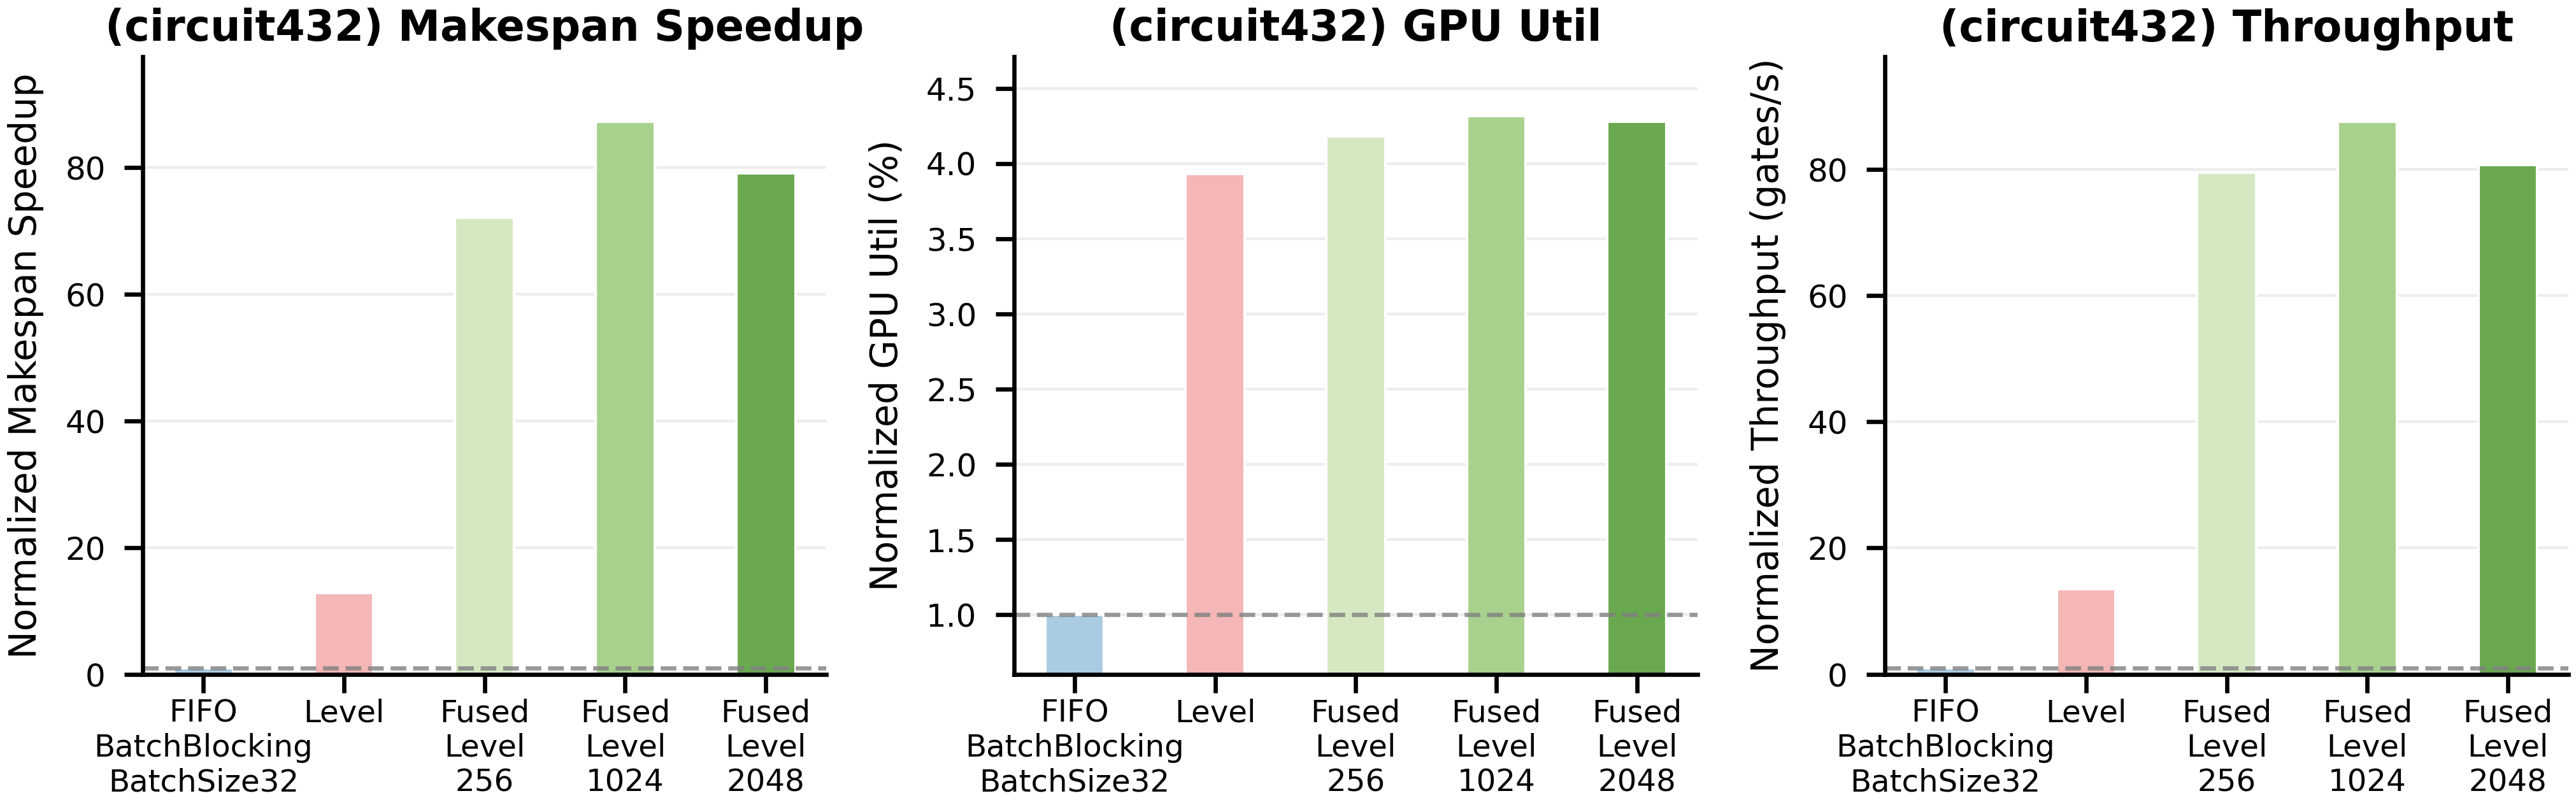
\includegraphics[width=0.43\textwidth]{report_c432_level_summary.png}\hspace{0.055\textwidth}
  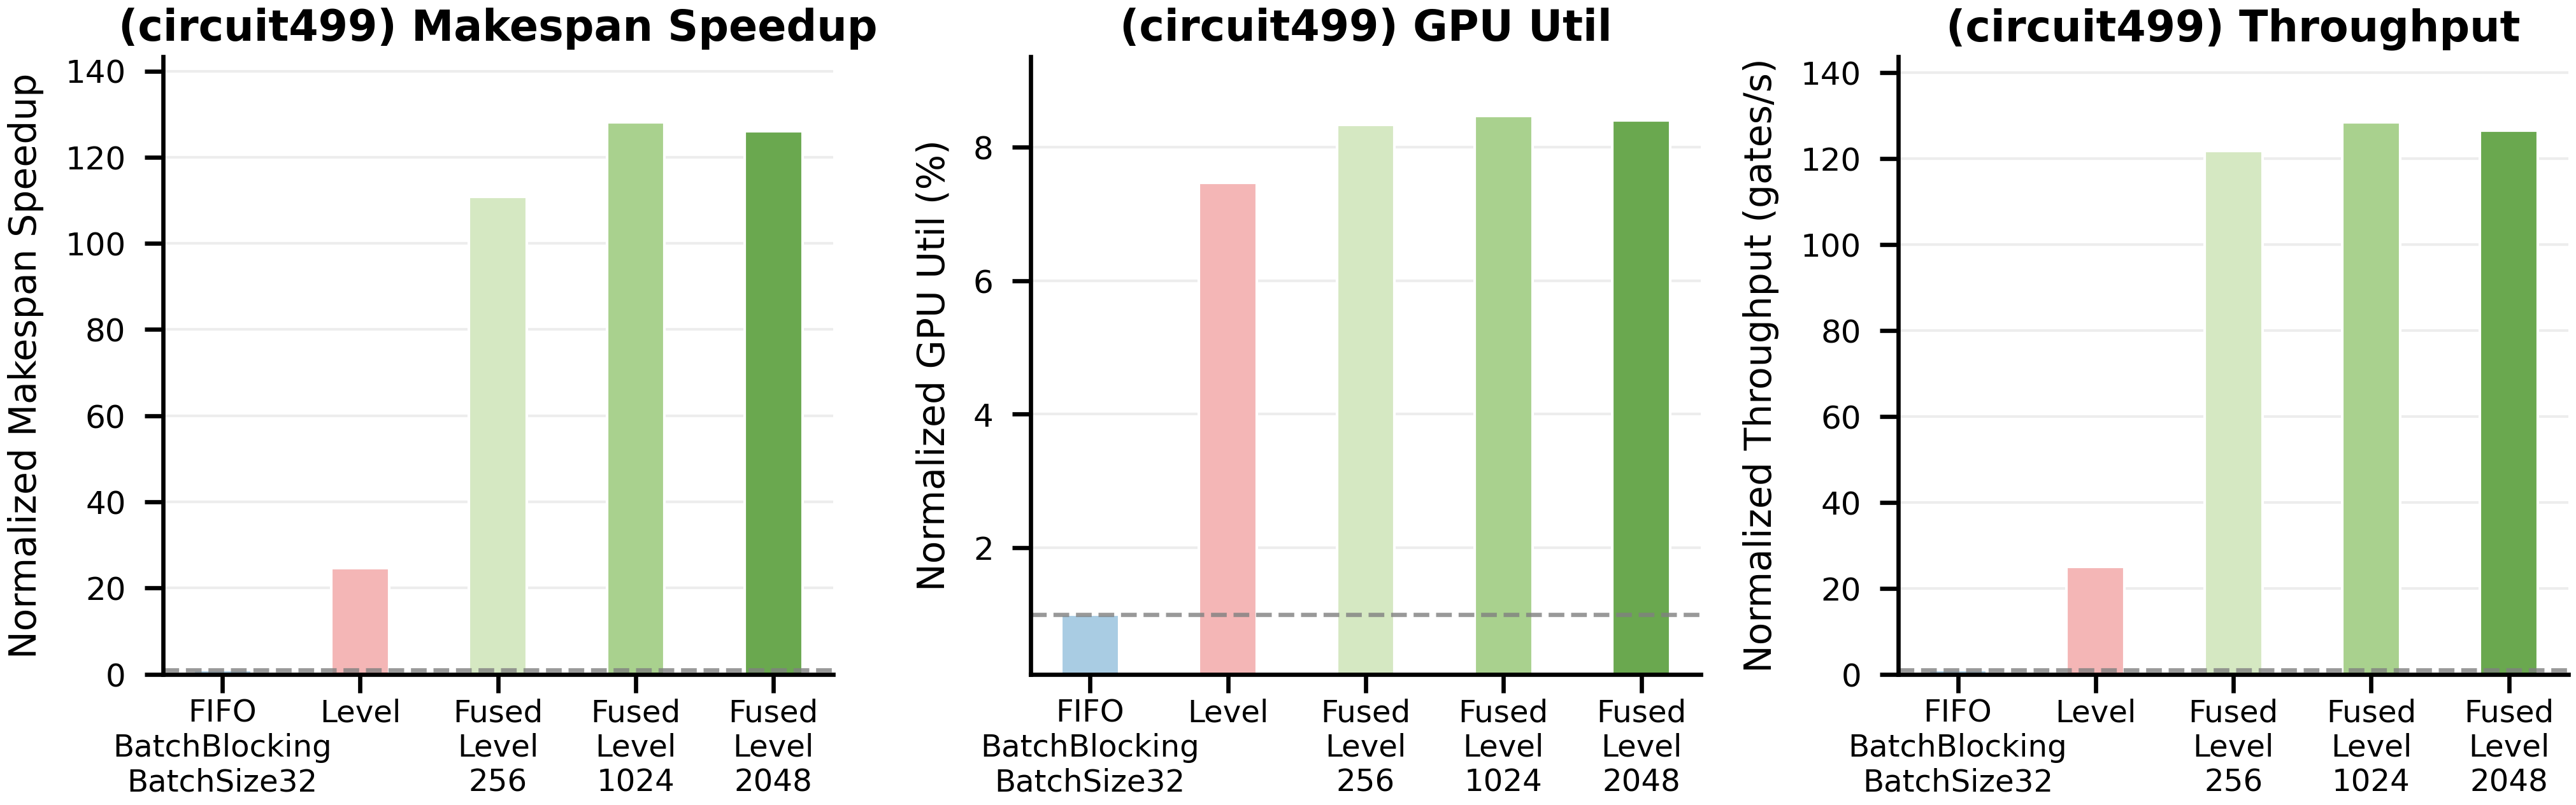
\includegraphics[width=0.43\textwidth]{report_c499_level_summary.png}
  \par\vspace{0.5pt}
  {\small (a) small circuits}
  \par\vspace{5pt}
  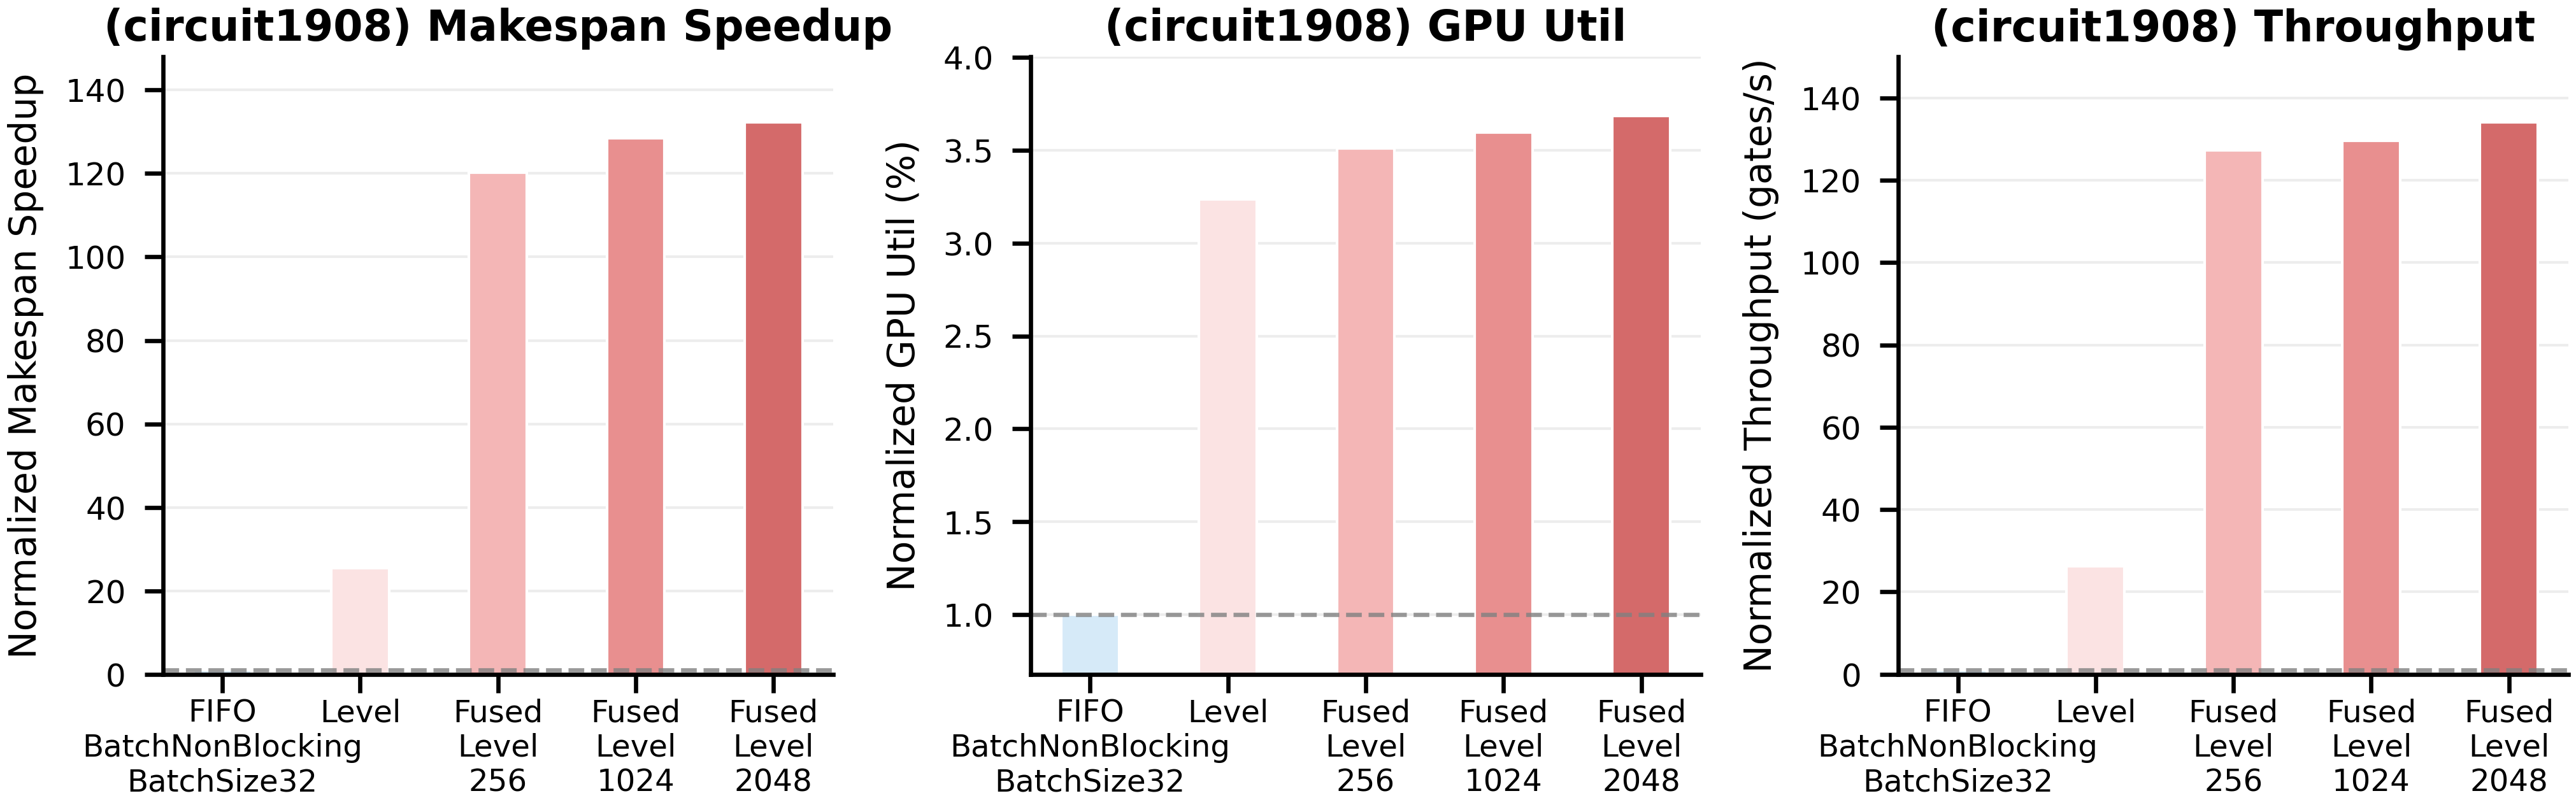
\includegraphics[width=0.43\textwidth]{report_c1908_level_summary.png}\hspace{0.055\textwidth}
  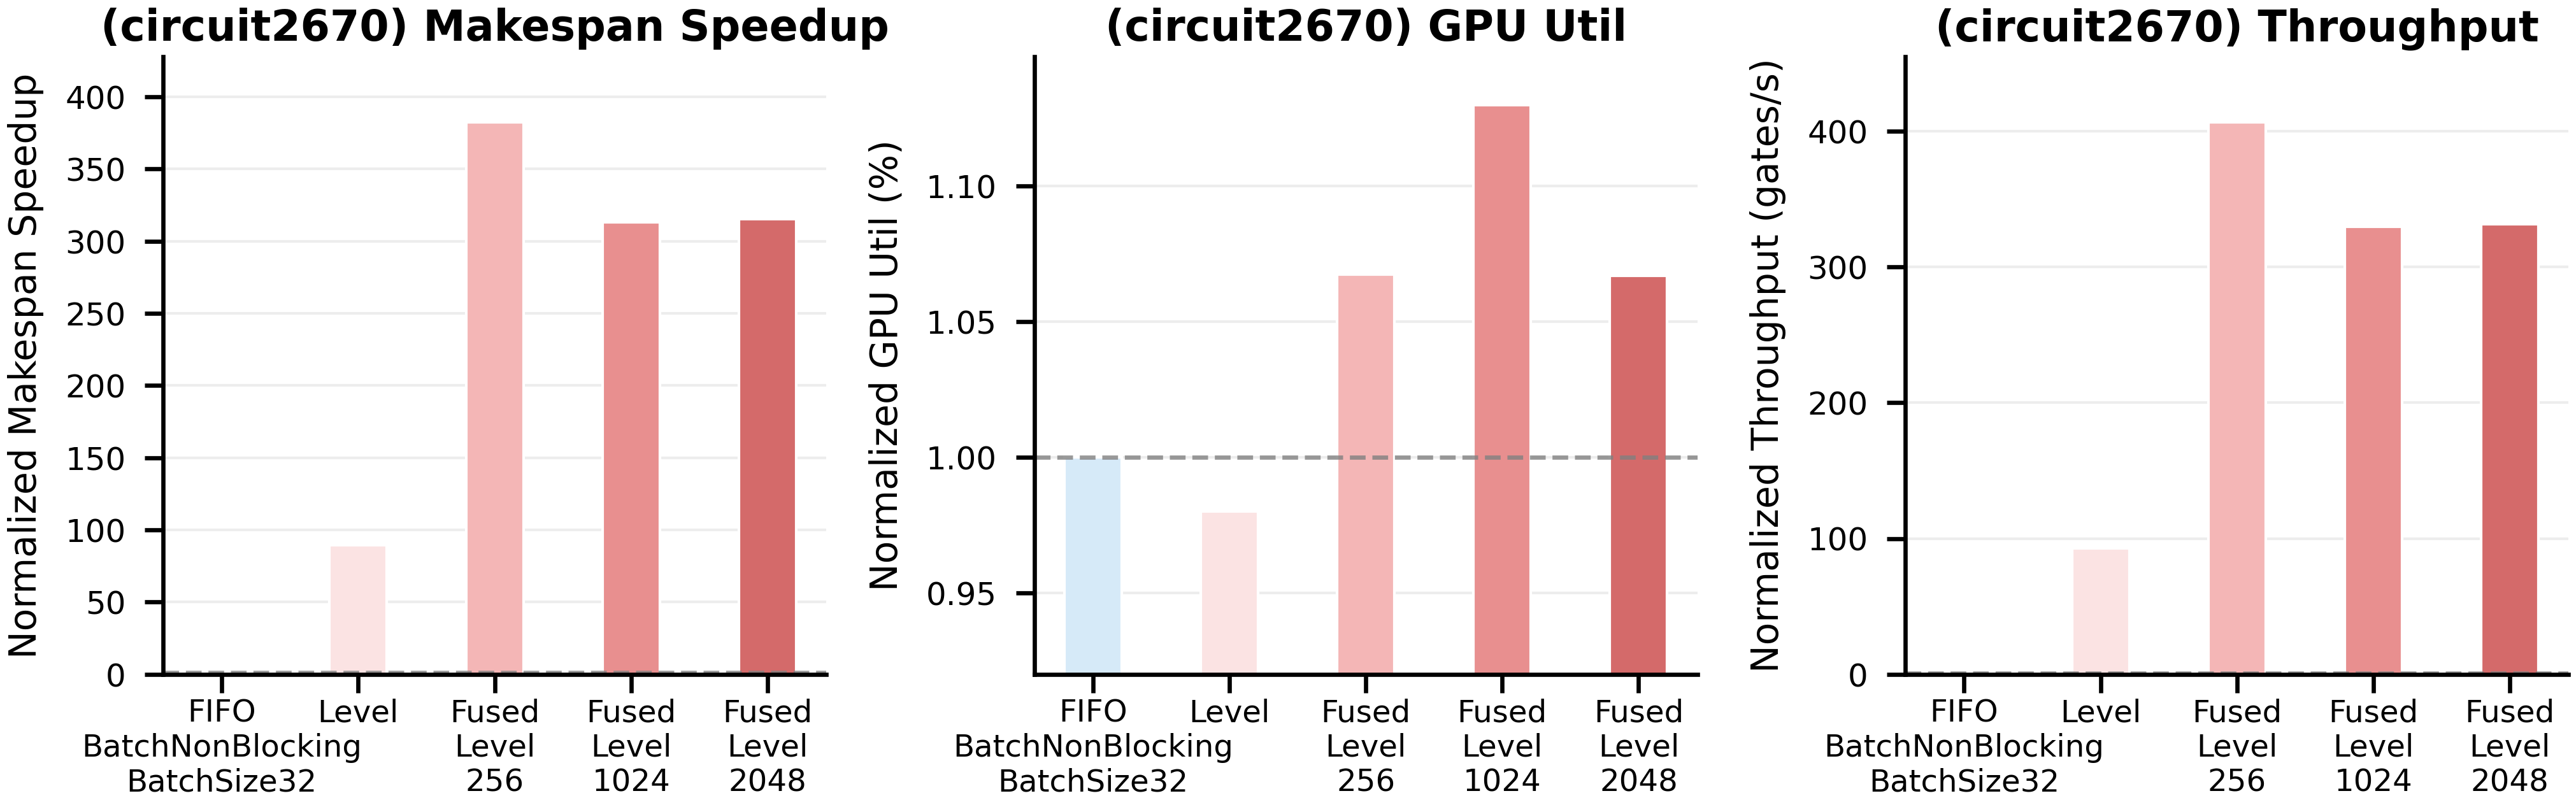
\includegraphics[width=0.43\textwidth]{report_c2670_level_summary.png}
  \par\vspace{0.5pt}
  {\small (b) medium circuits}
  \par\vspace{5pt}
  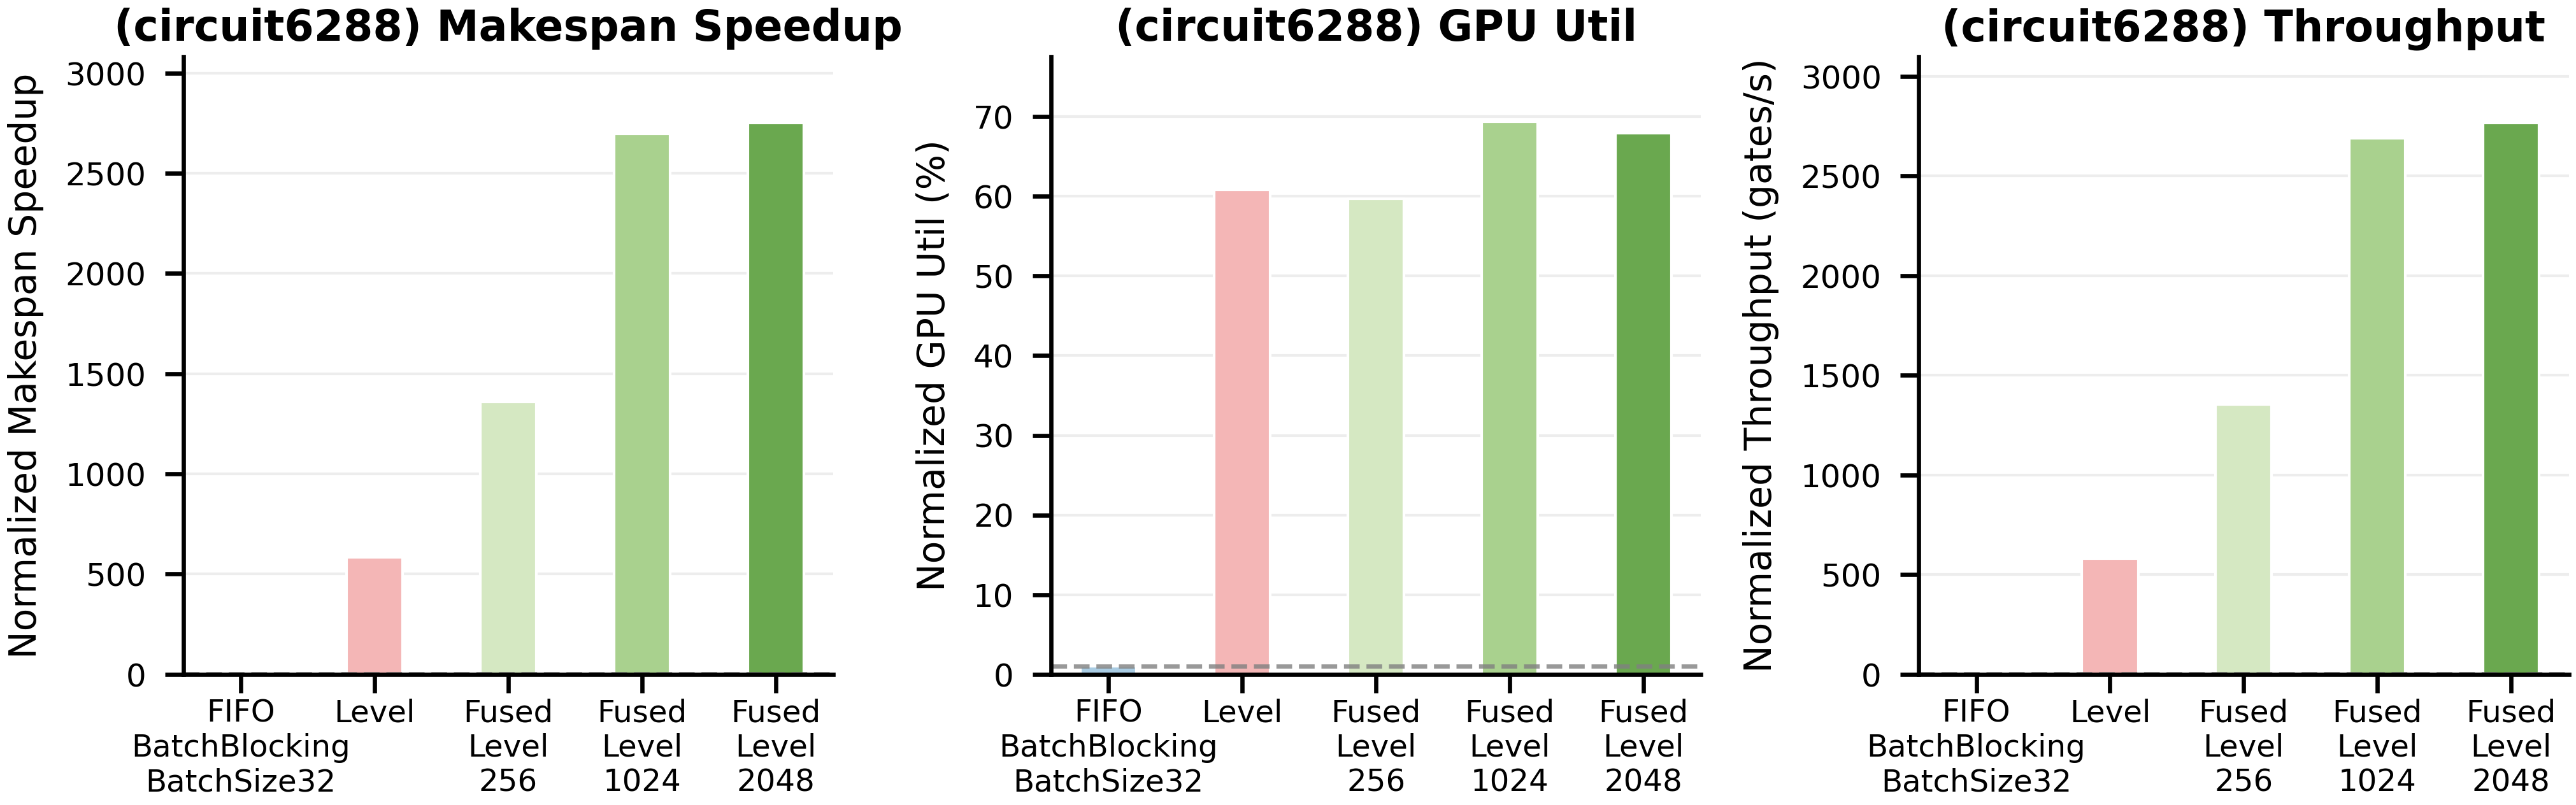
\includegraphics[width=0.43\textwidth]{report_c6288_level_summary.png}\hspace{0.055\textwidth}
  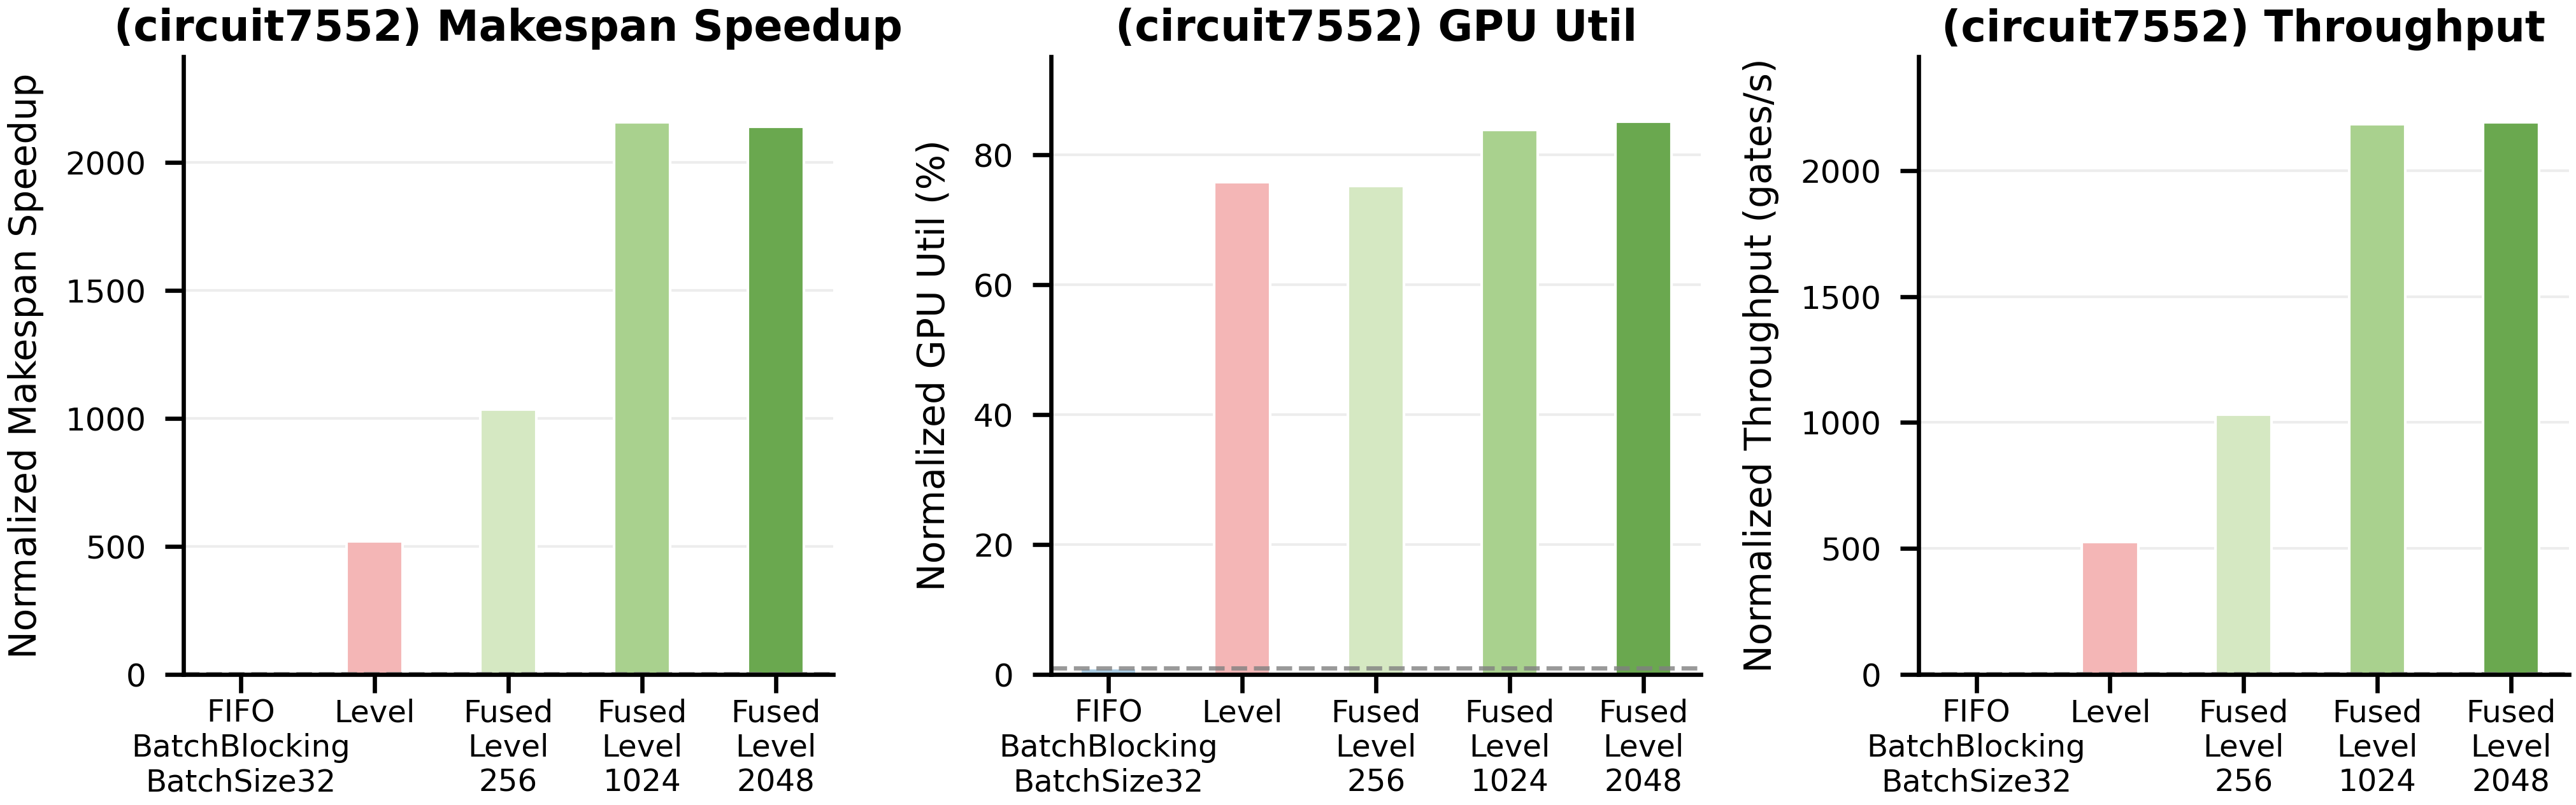
\includegraphics[width=0.43\textwidth]{report_c7552_level_summary.png}
  \par\vspace{0.5pt}
  {\small (c) large circuits}
  \caption{Levelization and fused-level execution across representative small, medium, and large circuits. Each bar is normalized to the FIFO batch non-blocking baseline with batch size 32.}
  \label{fig:levelization}
\end{figure*}

Levelization changes the execution granularity. Instead of selecting ready gates to form batches, it executes the circuit by topological levels. This reduces the number of scheduling units and uses the natural parallelism within each level. In our experiments, levelization significantly outperforms previous gate-level scheduling methods across small, medium, and large circuits. Using FIFO BatchNonBlocking with batch size 32 as the baseline, levelization achieves about 15x makespan speedup on small circuits and about 500x speedup on large circuits, with speedup increasing as circuit size grows. The main reasons are as follows. First, each logic operation is extremely lightweight, so even a small amount of host-side scheduling and launch overhead can noticeably affect total runtime. By packing gates into level tasks, levelization reduces the number of scheduling decisions and kernel launches. Second, as discussed above for gate-level scheduling, after a batch completes, the runtime must update dependencies for every completed gate, which is still an individual task, and the current implementation checks dependency relationships at gate granularity. This repeated host-side bookkeeping is included in makespan, wait time, and turnaround time. In contrast, with levelization, once a level completes, the runtime only needs to unlock the next level task instead of repeatedly processing dependency updates for each gate. This largely removes host-side dependency maintenance. The low GPU utilization observed in some gate-level batch results also supports this explanation: the GPU is idle for most of the wall-clock time, while the host spends time on scheduling and dependency bookkeeping. This also explains why \texttt{batch\_size = 512} can still perform much worse than levelization, even when no individual level is wider than 512 gates.

The main weakness of levelization is narrow tail levels. Many circuits have wide early levels but many later levels containing only a few gates. Launching one kernel per narrow level provides little GPU work per launch, so host-side launch overhead can dominate runtime. Therefore, the effectiveness of levelization depends on the level width distribution of the circuit.

\subsection{Fused Levelization}
\label{sec:fused-levelization}
Fused levelization directly targets the narrow-tail problem. By executing consecutive small levels inside one kernel, it reduces repeated host-side launches and synchronization. We compare fusion thresholds of 256, 1024, and 2048. With a threshold of 256, the results already show a clear improvement. Beyond a certain fusion size, most small levels are already merged, so further increasing the threshold provides little additional benefit.

\section{Weakness and Future Work}
This project has several limitations. First, GPU utilization is measured using host-side active intervals, not profiler-level SM occupancy. Second, the executor is a simplified course-project backend rather than a full industrial simulator. Third, the fused-level threshold is empirical and depends on GPU architecture, memory behavior, and circuit structure.

Based on our experiments, the most important observation is that levelization provides a large improvement for circuit graph execution. After reviewing related work, we believe that levelization and graph partitioning are more suitable directions for circuit graph execution than increasingly fine-grained GPU scheduling policies. Recent heterogeneous task-graph simulation work such as TaroRTL also suggests that circuit simulation benefits from explicit task-graph structure rather than only local ready-queue ordering \cite{10.1007/978-3-031-69583-4_11}. Future work should therefore focus on improving levelized execution and exploring partition-based execution. For levelization, profiling tools such as \texttt{nvprof} can be used to search for better fusion thresholds, and CUDA Graphs or conditional CUDA Graphs may further reduce repeated launch overhead. For partitioning, the circuit could be divided into subgraphs that balance parallelism, dependency depth, and GPU occupancy, possibly using replication-aided partitioning techniques.

\section{Conclusion}
This project compares several scheduling policies and execution granularities for GPU logic simulation. Gate-level scheduling policies can affect wait time and dependency progress, but their effectiveness is limited by the extremely low cost of individual gate operations, large launch overhead, and frequent dependency-update latency. Levelization reduces scheduling granularity by executing gates level by level, removes much of the per-gate host-side scheduling and dependency-update overhead, and significantly improves multiple metrics. However, narrow tail levels can still cause inefficient small kernel launches. Fused levelization reduces this overhead by executing consecutive small levels inside one kernel. Overall, for fine-grained dependency-heavy GPU applications such as logic simulation, choosing the right execution granularity is often more important than designing a more complex ready-queue scheduler.

\bibliographystyle{ACM-Reference-Format}
\bibliography{base}

\end{document}
